\section{Motivating scenario}
\label{sec:motivatingscenario}

In this section we present a motivating scenario that we use to illustrate the preliminary definitions introduced in the previous section and that we will use to present our approach. This scenario is a set three DSLs.The first one is the classical Logo that has been historically used it in education. The second one is a DSL for expressing flow charts. Finally, the third one is a DSL for expressing simple state machines.

Figure \ref{fig:motivating-example} shows the metamodels corresponding to each of the DSLs. Although each language is independent, it is clear that there are certain commonalities that represent potential reuse. The most important commonality is highlighted in yellow and corresponds to the constructs for expressing simple arithmetic expressions. The three DSLs of the scenario use the same constructs. 

\begin{figure}
\centering
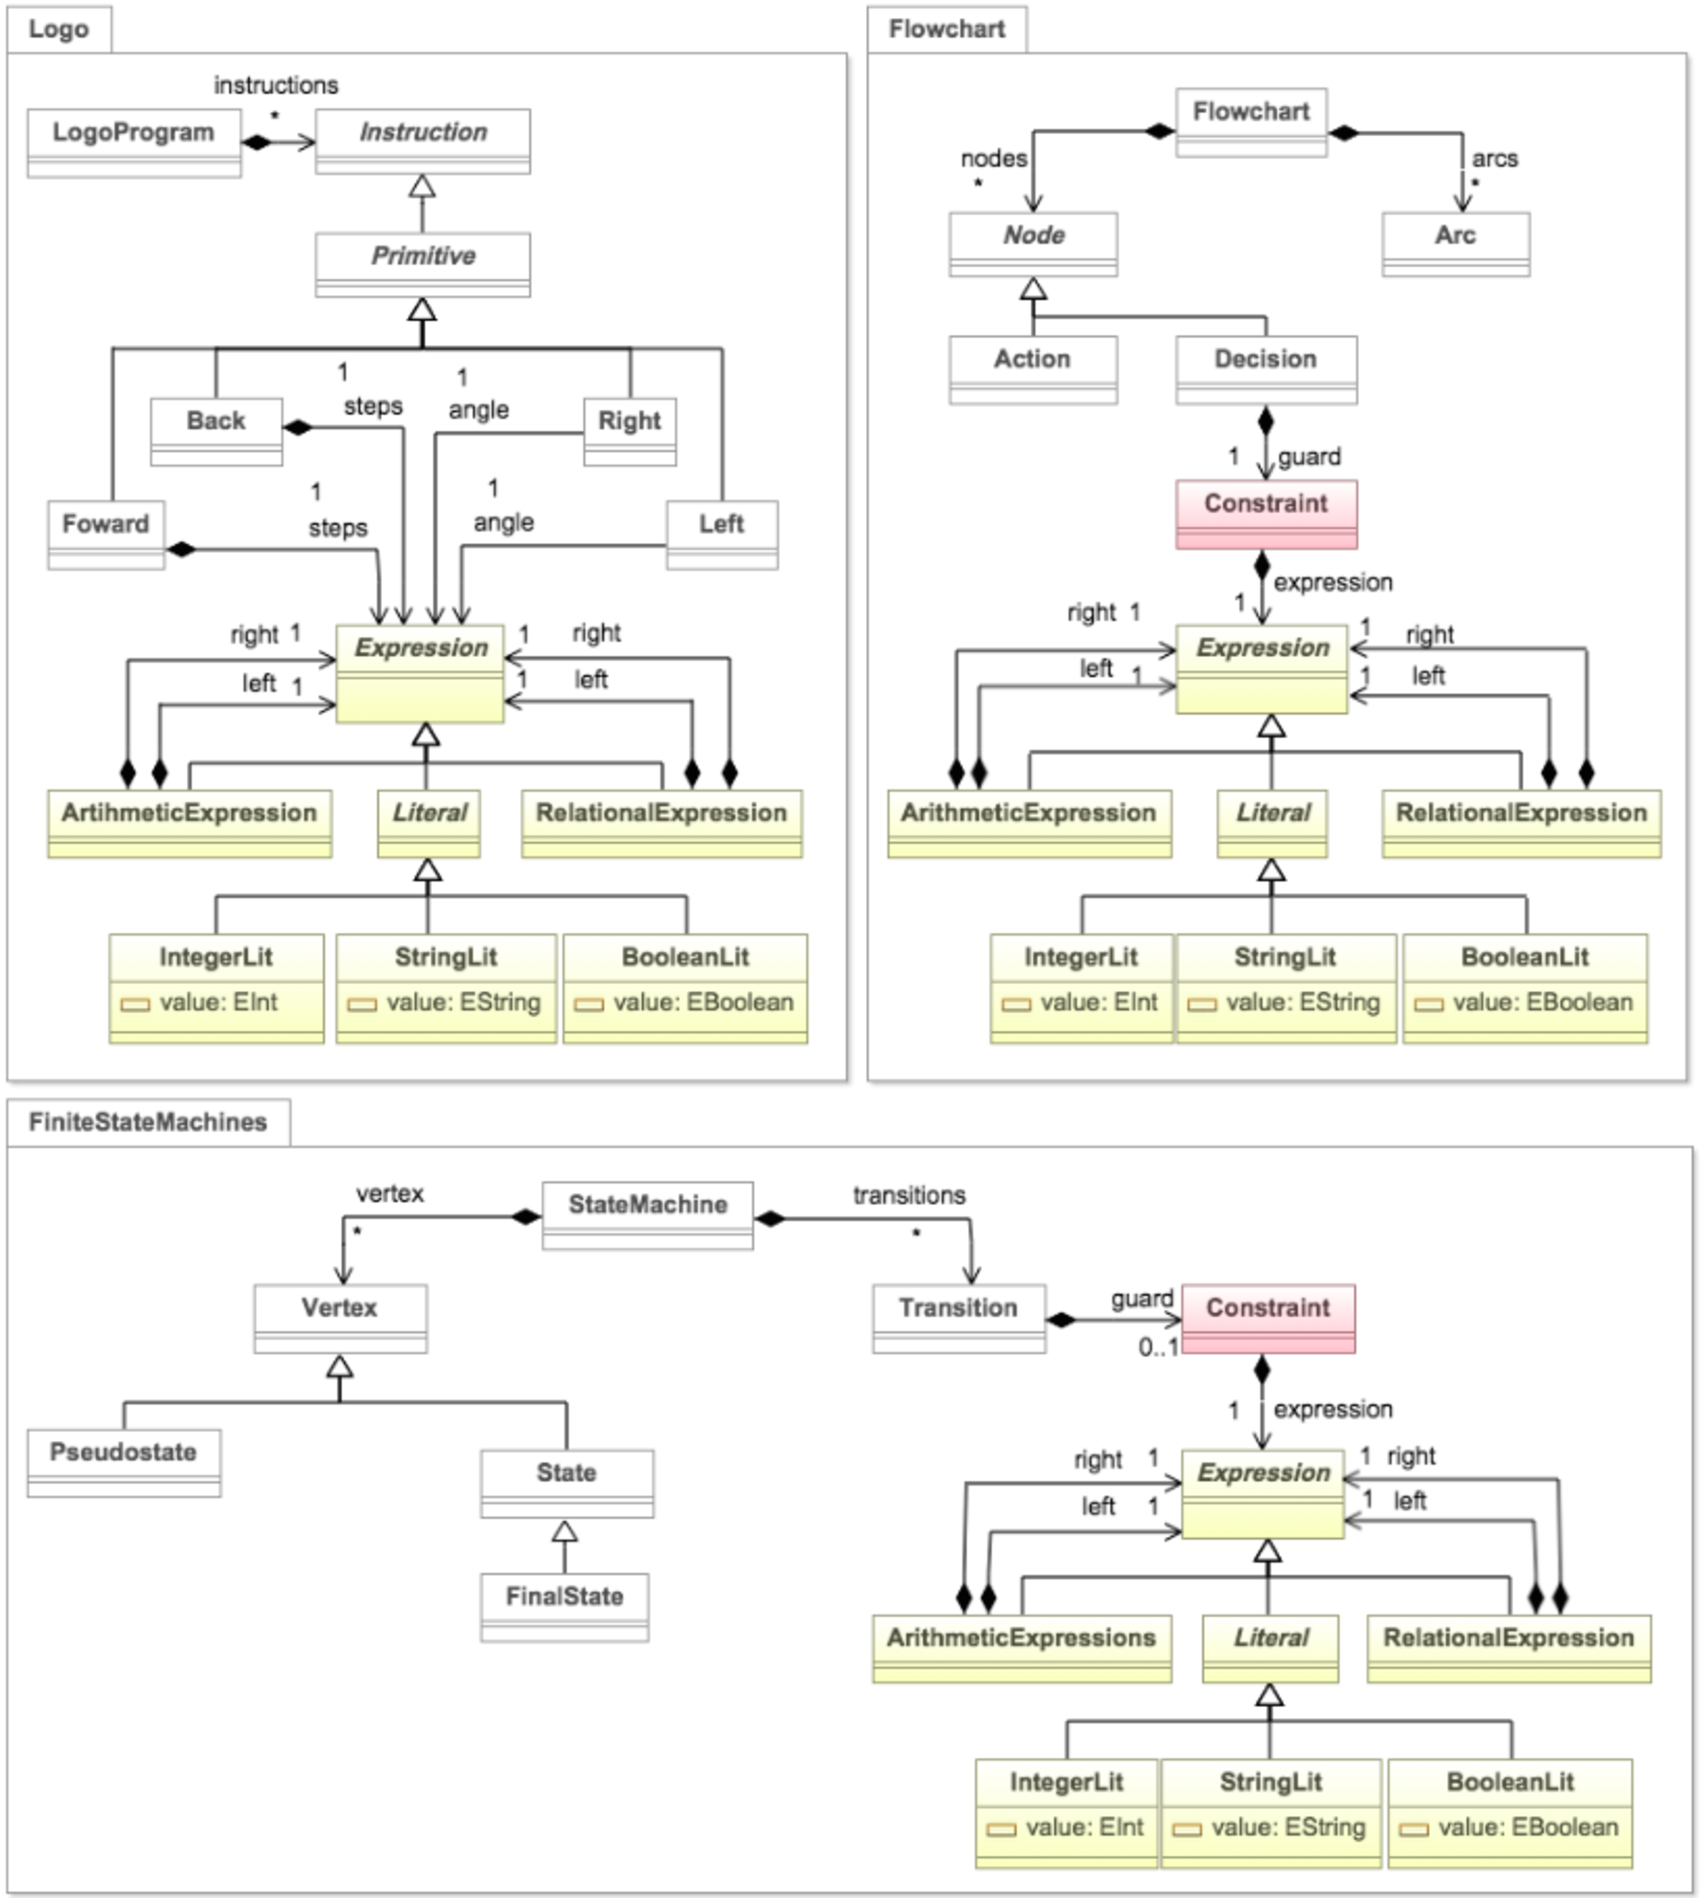
\includegraphics[width=1.05\linewidth]{images/motivating-example.pdf}
\caption{Different relationships between DSL domains}
\label{fig:motivating-example}
\end{figure}